

\section{“经典”\trHamiltonianSystem}
\label{sec:classical-hamiltonian-systems}

\hzsync{theorem}{6}
\hzsync{proposition}{4}

一个具有 $n$ 个\textbf{\trDegreesOfFreedom}（degrees of freedom）的\textbf{\trConservativeSystem}%
（conservative system），其位置是所谓\textbf{\trConfigurationSpace}%
（configuration space）中的点，我们假定后者是一个 $n$ 维\trSmooth\trManifold{}%
$N$。该系统的运动，在\textbf{\trLagrange{}力学}（Lagrangian mechanics）的%
框架中，由定义在 $N$ 的\textbf{\trTangentBundle}（tangent bundle）$TN$ 上的%
一个\textbf{\trLagrange{}量}（Lagrangian）$L$ 所确定。这个 $2n$ 维%
\trManifold{}称为该系统的\trPhaseSpace。在我们的\textbf{\trHamiltonian{}力学}%
（Hamiltonian mechanics）框架中，系统的运动由定义在 $N$ 的%
\textbf{\trCotangentBundle}（cotangent bundle）$T^{*}N$ 上的一个%
\trHamiltonianFunction{} $H$ 所确定。这是\trSymplecticManifold{}的基本例子。%
它装备着一个\textbf{典范\trSymplecticStructure}（canonical symplectic
structure），我们将首先对此作一回顾。

若 $N$ 是维数为 $n$ 的任一\trManifold，而 $T_{x}N$ 是点 $x\in N$ 处的%
\trTangentSpace，则把它的\trDual{}空间——所谓的\textbf{\trCotangentSpace}%
（cotangent space）——记作 $T^{*}_{x}N$。它是定义在向量空间 $T_{x}N$ 上的%
诸\trLinear{}形式所成的空间。全体\trCotangentSpace{}之并称为 $N$ 的%
\trCotangentBundle，并记作
\[
T^{*}N\ =\ \bigcup_{x\in N}T^{*}_{x}N.
\]
集合 $M=T^{*}N$ 中的一点 $\alpha$ 是某点 $x\in N$ 处\trTangentSpace{} $T_{x}N$%
上的一个\trLinear{}形式 $\alpha_{x}$，对 $M$ 中的点我们有时使用记号
\[
\xi\ =\ (x,\xi_{x})\ \in\ T^{*}N
\]
来表示。通过引入局部坐标，人们可以把 $T^{*}N$ 看作一个维数为 $2n$ 的可微%
\trManifold，如下进行。若 $(x_{1},\dots,x_{n})$ 是 $N$ 中的局部坐标，则%
\trOneForm{} $\alpha\in T^{*}_{x}N$ 可表示为 $\alpha=\sum_{j=1}^{n}y_{j}\,dx_{j}$，%
它具有坐标 $(y_{1},\dots,y_{n})$，而 $(x_{1},\dots,x_{n},y_{1},\dots,y_{n})$%
合起来便构成 $T^{*}N$ 中的局部坐标。在这些坐标中，现在可以定义 $T^{*}N$ 上%
特殊的\trOneForm{} $\lambda$
\begin{equation}\label{eq:liouville-local}
\lambda\ =\ \sum_{j=1}^{n}y_{j}\,dx_{j},
\end{equation}
它迄今为止只有一个局部的意义。值得注意的是，上述形式 $\lambda$ 在 $T^{*}N$%
上有一个整体的解释。由于 $T^{*}N$ 的一个点由点 $x\in N$ 处的一个\trOneForm{}%
$\xi$ 所表示，我们对每个向量 $V\in T_{x}N$ 都可以构成 $\xi(V)$。要在 $T^{*}N$%
上定义一个\trOneForm{}——比如说 $\beta$——就必须对 $T^{*}N$ 的每个切向量%
$X$ 给出它的值 $\beta(X)$。若 $X$ 是点 $\xi\in T^{*}N$ 处的这样一个切向量，%
则可以利用形式 $\xi$ 自身把它定义为\trLinear{}\trFunctional
\begin{equation}\label{eq:tautological-form}
\lambda_{\xi}(X)\ =\ \xi\bigl(d\pi X\bigr),\qquad X\in T_{\xi}\bigl(T^{*}N\bigr)
\end{equation}
这里\trProjection{} $\pi:T^{*}N\to N$ 把每个 $\xi\in T^{*}N$ 对应到它的基点 $x\in N$，%
从而 $d\pi$ 把 $\xi$ 处的\trTangentSpace{} $T_{\xi}\bigl(T^{*}N\bigr)$ 映满点%
$x$ 处的\trTangentSpace{} $T_{x}N$。$T^{*}N$ 上的这个\trOneForm{} $\lambda$%
有时被称为 $T^{*}N$ 上的\textbf{\trTautologicalForm}（tautological form），因为它由其%
自身来定义。容易验证：在上述局部坐标中，形式 \eqref{eq:tautological-form}%
与形式 \eqref{eq:liouville-local} 相一致。由表达式 \eqref{eq:liouville-local}%
我们得到
\[
d\lambda\ =\ \sum_{j=1}^{n}dy_{j}\wedge dx_{j}
\]
并得出结论：整体地，$\omega=d\lambda$ 是 $T^{*}N$ 上一个\trClosed{}且%
\trNondegenerate{}的\trTwoForm，因而是一个\trSymplecticForm。它称为 $T^{*}N$%
上的典范\trSymplecticStructure。$T^{*}N$ 上的典范\trOneForm{} $\lambda$ 称为\textbf{\trLiouville{}形式}%
（Liouville form）。顺带指出，$\lambda$ 具有如下特定的性质：对 $N$ 上的每个%
\trOneForm{} $\beta$ 都有
\[
\beta^{*}\lambda\ =\ \beta
\]
这里\trOneForm{} $\beta$ 被看作一个\trSection{} $\beta:N\to T^{*}N$。该证明来自%
观察 $\pi\circ\beta=id$ 于 $N$ 上：考虑 $\lambda$ 的定义并利用\trChainRule，%
我们发现
\[
\bigl(\beta^{*}\lambda\bigr)_{x}\ =\ \lambda_{(x,\beta_{x})}(d\beta)_{x}\ =\ %
\beta_{x}\circ d\pi_{(x,\beta_{x})}\circ(d\beta)_{x}\ =\ \beta_{x}
\]
正如所断言的。

经典力学系统由 $\bigl(T^{*}N,d\lambda\bigr)$ 上的\trHamiltonianFunction{}描述，%
后者由\textbf{\trKineticEnergy}（kinetic energy）与\textbf{\trPotentialEnergy}（potential energy）之和%
给出。\trKineticEnergy{}由\trConfigurationSpace{}上的一个\trRiemann{}度量 $k$ 定义，这个度量%
使每一点 $x\in N$ 联系一个\trSymmetric\trBilinear{}形式 $k_{x}(v,w)$（$v$,%
$w\in T_{x}N$），它是正的。这一度量定义了一个丛\trIsomorphism{}%
$\gamma:TN\to T^{*}N$：$\gamma(v)(w)=k(v,w)$，由它经
\[
K(\xi,\eta)\ =\ k\left(\gamma^{-1}(\xi),\gamma^{-1}(\eta)\right).
\]
在\trCotangentBundle{} $T^{*}N$ 上诱导出相应的\trRiemann{}度量 $K$。\trPotentialEnergy{}由\trConfigurationSpace{}%
上的一个\trSmooth{}函数 $V:N\to\R$ 表示。于是在 $T^{*}N$ 上\trHamiltonianFunction{}%
$H$ 定义为
\begin{equation}\label{eq:classical-hamiltonian}
H(\xi)\ =\ K(\xi)\ +\ V\bigl(\pi(\xi)\bigr)\,,\qquad\ \xi\in T^{*}N.
\end{equation}
在上述局部坐标中，我们有公式：
\begin{equation}\label{eq:local-formulae}
\begin{aligned}
H\ &=\ K(x,y)+V(x)\\
\lambda\ &=\ \sum_{j=1}^{n}y_{j}\,dx_{j}\\
X_{H}\ &=\ \sum_{j=1}^{n}\left(\frac{\partial K}{\partial y_{j}}\frac{\partial}{\partial x_{j}}-\frac{\partial H}{\partial x_{j}}\frac{\partial}{\partial y_{j}}\right)\\
\lambda\bigl(X_{H}\bigr)\ &=\ \sum_{j=1}^{n}y_{j}\,\frac{\partial K}{\partial y_{j}}\ =\ 2K\,,
\end{aligned}
\end{equation}
其中\footnote{原书公式 (4.10) 第三行首项印作 $\partial K/\partial y_{j}$ 而次项印作 $\partial H/\partial x_{j}$，记号混用（$V$ 不依赖 $y$，二者相等），此处照录原书面貌。——译者注} $K(x,y)=\tfrac{1}{2}\bigl\langle S(x)y,y\bigr\rangle$，而 $S(x)$ 为一个%
\trPositiveDefinite{}矩阵。

若 $\xi(t)$ 是\trHamiltonianVectorField{} $X_{H}$ 的一个含于\trInvariant%
\trEnergySurface
\begin{equation}\label{eq:SE-energy-level}
S\ =\ \Bigl\{\,\xi\ \Bigm|\ H\ =\ K+V\ =\ E\Bigr\},
\end{equation}
之中的解，则该系统在\trConfigurationSpace{}中的几何运动由%
$x(t)=\pi\bigl(\xi(t)\bigr)\in N$ 给出，这里 $\pi:T^{*}N\to N$ 是\trProjection。由于%
$K\geq0$，它被限制在子集
\begin{equation}\label{eq:NE-confined}
N_{E}\ =\ \Bigl\{\,x\in N\ \Bigm|\ V(x)\ \leq\ E\Bigr\}.
\end{equation}
之中。若 $E<\max V$，则此集合是一个 $n$ 维\trManifold，并且——只要 $S$ 是一张%
\trRegular\trEnergySurface——具有\trSmooth{}的\trBoundary{} $\partial N_{E}=\bigl\{V(x)=E\bigr\}$。%
的确，在 $K=0$ 处我们也有 $\tfrac{\partial}{\partial y}K=0$，故在 $V(x)=E$ 上%
必有 $\tfrac{\partial}{\partial x}V(x)\neq0$。然而，若 $E>\max V$，则%
$N_{E}=N$ 是整个\trConfigurationSpace，且 $K>0$ 于 $S$ 上。于是%
$\lambda\bigl(X_{H}\bigr)=2K>0$ 于 $S$ 上，从而我们看到 $S$ 是一张%
\trContactType\trHypersurface，其\trContactStructure{}借助\trLiouville{}形式%
$\lambda$ 来定义。如果在 $T^{*}N$ 中 $S$ 有一个\trNeighborhood{} $U$ 使%
\trCapacity{} $c_{0}(U)$ 有限，我们便可以断定 $S$ 容纳一条%
\trClosedCharacteristic。遗憾的是，关于\trCotangentBundle{}上的特殊%
\trCapacity{} $c_{0}$ 一无所知，唯有\trTorus{}这一特殊情形除外——它将在%
后面处理。

$S$ 上的\trPeriodicSolution{}业已借助几何的想法找到，下面我们对此作一简要%
说明。假设 $E>\max V$，则有
\[
T^{*}N_{E}\ =\ T^{*}N
\]
并且可以在 $T^{*}N$ 上定义特殊的\trRiemann{}度量 $G$：
\[
G(\xi)\ =\ \frac{K(\xi)}{E-V\bigl(\pi(\xi)\bigr)}\,,\qquad\ \xi\in T^{*}N.
\]
这就是所谓的\textbf{\trJacobi{}度量}（Jacobi metric）。现在我们有两个%
\trHamiltonianFunction，即 $H$ 与 $G$，它们把 $S$ 描述为\trRegular%
\trEnergySurface
\[
S\ =\ \bigl\{H(\xi)=E\bigr\}\ =\ \bigl\{G(\xi)=1\bigr\}.
\]
于是，相应的诸\trHamiltonianVectorField{}是平行的：在 $S$ 上%
$X_{H}=\rho X_{G}$，其中 $\rho$ 是定义在 $S$ 上的一个无处为零的函数，而且%
实际上在局部坐标中容易把它算出。人们发现，在 $S$ 上
\[
X_{H}\ =\ K\cdot X_{G}\qquad\text{于}\quad S.
\]
从而，\trVectorField{} $X_{H}$ 与 $X_{G}$ 在 $S$ 上经\trReparametrization{}后%
具有相同的\trOrbit。几何上看，\trVectorField{} $X_{G}$ 生成由 $T^{*}N$ 上的%
\trRiemann{}度量 $G$ 所定义的\textbf{\trGeodesic{}流}（geodesic flow）。%
\trFlow{}线的\trProjection{} $\pi\bigl(\xi(t)\bigr)$ 是\trConfigurationSpace{} $N$ 中的%
一条\trGeodesic，也就是说，它在两点之间局部地极小化长度，这里长度是关于%
$TN$ 上的度量 $g$ 来量的，而 $g$ 由下式给出：
\[
g_{x}(v,w)\ =\ \bigl(E-V(x)\bigr)^{-1}k_{x}(v,w)\,,\qquad\text{其中}\ \ %
v,w\in T_{x}N.
\]
我们看到，$T^{*}N$ 上\trRiemann{}度量 $G$ 的诸\trGeodesic{}经\trReparametrization{}后%
与 $X_{H}$ 在 $S$ 上的诸解相一致。当然，这只在特定的\trEnergySurface{} $S$ 上%
成立。这一事实通称\trEuler-\trMaupertuis-\trJacobi{}原理。它把「求\trHamiltonianVectorField{}%
在 $S$ 上的解」这一动力学问题化归为「求 $N$ 上\trJacobi{}度量的\trGeodesic」这一%
几何问题——一个有着丰富历史的问题。

回忆一下：若 $N$ 不是\trSimplyConnected{}的（例如一个\trTorus），则可以考察一个%
非平凡\textbf{\trHomotopy{}类}（homotopy class）中的\trClosed\trCurve{}族，%
并由此得到一条长度最短的\trClosed\trGeodesic。这一点早已为\trHadamard（1889）所知。%
在技术上，这一方法要求长度\trFunctional{}在\trLoop{}的\trSubspace{}上达到它的%
极小，这是一个分析问题，D.~\trHilbert（1890）清楚地看到并着手处理了它，%
见 [112]。在\trSimplyConnected{}的\trRiemann\trManifold{} $N$ 上寻找%
\trClosed\trGeodesic{}是一个困难而有趣的课题。在这种情形，诸\trGeodesic{}不能%
作为极小点、而要作为长度\trFunctional{}的\trSaddlePoint{}来寻找，此时要利用%
基础\trManifold{} $N$ 的\trLoopSpace{}的\trTopology。\trBirkhoff{}利用一个%
\trMinimax{}原理在二维\trSphere{}上确立了一条\trClosed\trGeodesic，这一原理%
后来引出了关于\trCriticalPoint{}的\trLjusternik-\trSchnirelman{}理论。大约在%
同一时期发展起来的\trMorseTheory{}则起源于\trGeodesic{}的存在性问题。把%
\trBirkhoff{}的想法推广到高维，\trLjusternik{}与\trFet{}在 1951 年 [81] 证明了：%
每张\trCompact\trRiemann\trManifold{} $(N,g)$ 都具有一条\trClosed\trGeodesic。取%
\trJacobi{}度量，由这一几何结果便立即推出：只要 $N$ \trCompact{}且%
$E>\max V$，上面的\trEnergySurface{} $S$ 就具有一条\trClosedCharacteristic。

在 $E<\max V$ 的情形，\trClosed\trGeodesic{}理论不能直接适用，因为此时\trManifold{}%
$N_{E}$ 具有\trBoundary{} $\partial N_{E}$，而\trJacobi{}度量正是在该边界处趋于无穷的。%
尽管有这一分析上的困难，S.~V.~\trBolotin{}[29] 在 1978 年还是成功地使用了几何%
方法，用以证明：

\begin{theorem}\label{thm:bolotin-classical-system}
设 $N$ 为任一\trSmooth\trManifold，并设 $H:T^{*}N\to\R$ 描述形如%
\eqref{eq:classical-hamiltonian} 的一个经典系统。那么，每张\trCompact{}且%
\trRegular{}的\trEnergySurface{} $S_{E}$ 都具有 $X_{H}$ 的一个%
\trPeriodicSolution。
\end{theorem}

本定理推广了 H.~\trSeifert{} [193] 于 1948 年的一个较早结果，后者要求%
$N_{E}$ \trHomeomorphic{}于一个 $n$ 维\textbf{\trCell}（$n$-cell）。1917 年，%
\trBirkhoff{}对 $N_{E}=S^{2}$ 的情形证明了这一论断。

利用几何方法，\trBolotin{}的结果后来又被 H.~\trGluck{}与 W.~\trZiller（1983）[106] 以及%
更晚的 V.~\trBenci（1984）[18] 重新发现。我们还应当提到：在 $\partial N_{E}%
\neq\emptyset$ 的情形，该定理所找到的\trPeriodicSolution{}是一条所谓的%
\textbf{\trBrakeOrbit}（brake orbit）。\trBrakeOrbit{}是指这样的\trOrbit：其在%
\trConfigurationSpace{} $N_{E}$ 中的运动 $\pi\bigl(\xi(t)\bigr)$ 在\trBoundary{}%
$\partial N_{E}$ 的不同点之间来回往返，而其余部分则穿行于\trInterior{}之中。%
应当注意，所考察的这些系统都是可逆的：若 $\xi(t)$ 是 $X_{H}$ 的一个解，则%
$-\xi(-t)$ 也是一个解，从而与\trConfigurationSpace{}中的运动%
$x(t)=\pi\bigl(\xi(t)\bigr)$ 相对应的、逆向行走的运动%
$x(-t)=\pi\bigl(-\xi(-t)\bigr)$ 同样对应于 $X_{H}$ 的一个解。当然，这一情形%
是人们从函数 $H(x,y)=\tfrac{1}{2}y^{2}+V(x)$ 的二维情形中所熟知的，正如下面%
的图所描绘的那样。

\noindent\begin{minipage}{\linewidth}
\centering
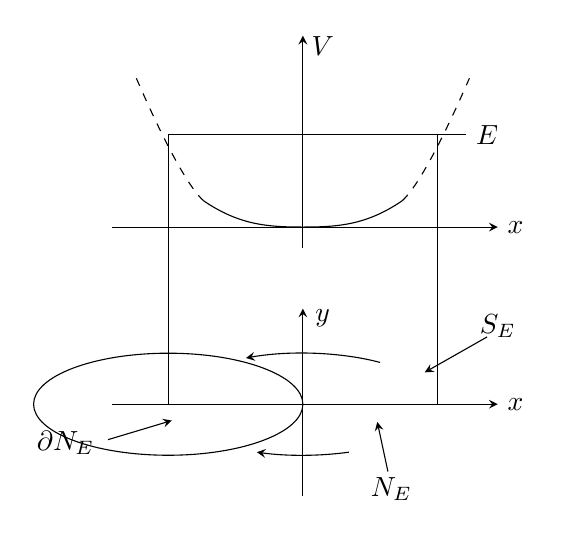
\begin{tikzpicture}[>=stealth,scale=0.9]
  \draw[->] (0,3.75) -- (0,6.75);%
  \node at (0.28,6.6) {$V$};
  \draw[->] (-2.7,4.05) -- (2.75,4.05);%
  \node at (3.0,4.05) {$x$};
  \draw[dashed] (-2.35,6.15) .. controls (-1.85,5.0) and (-1.55,4.55) .. (-1.4,4.42);%
  \draw (-1.4,4.42) .. controls (-0.9,4.08) and (-0.5,4.05) .. (0,4.05)
        .. controls (0.5,4.05) and (0.9,4.08) .. (1.4,4.42);%
  \draw[dashed] (1.4,4.42) .. controls (1.55,4.55) and (1.85,5.0) .. (2.35,6.15);%
  \draw (-1.9,5.35) -- (2.3,5.35);%
  \node at (2.6,5.35) {$E$};
  \draw[very thin] (-1.9,5.35) -- (-1.9,1.55);%
  \draw[very thin] (1.9,5.35) -- (1.9,1.55);%
  \draw[->] (0,0.25) -- (0,2.9);%
  \node at (0.28,2.76) {$y$};
  \draw[->] (-2.7,1.55) -- (2.75,1.55);%
  \node at (3.0,1.55) {$x$};
  \draw (-1.9,1.55) ellipse (1.9 and 0.72);%
  \draw[->] ([shift={(0,1.55)}]55:1.9 and 0.72)
        arc[start angle=55,end angle=115,x radius=1.9,y radius=0.72];%
  \draw[->] ([shift={(0,1.55)}]290:1.9 and 0.72)
        arc[start angle=290,end angle=250,x radius=1.9,y radius=0.72];%
  \node at (2.75,2.65) {$S_{E}$};
  \draw[->] (2.6,2.5) -- (1.72,2.0);%
  \node at (-3.35,1.0) {$\partial N_{E}$};
  \draw[->] (-2.75,1.05) -- (-1.85,1.32);%
  \node at (1.25,0.35) {$N_{E}$};
  \draw[->] (1.2,0.6) -- (1.05,1.3);%
\end{tikzpicture}

图 4.9
\end{minipage}

关于\trClosed\trGeodesic{}有许多结果，把它们应用于\trJacobi{}度量便导向%
\trEnergySurface{}的\trClosedCharacteristic。关于这些进展，我们请读者参阅%
\trKlingenberg{}的专著 [127] 与 V.~\trBangert{}的综述文章 [14]。我们应当指出：直到最近，%
V.~\trBangert{}[15] 与 J.~\trFranks{}[100] 才成功地在每张\trRiemann{}二维\trSphere{}上%
确立起无穷多条\trClosed\trGeodesic！

上面概述的几何方法只适用于含于一个\trCotangentBundle{}之中的很受限的一类%
\trHypersurface；我们愿意提到，C.~\trViterbo{}与 H.~\trHofer{}于 1988 年在%
[121] 中用一种颇为不同的分析方法证实了\trCotangentBundle{}情形的%
\trWeinstein{}猜想，如下：

\begin{theorem}[\trHofer-\trViterbo]\label{thm:hofer-viterbo-cotangent}
设 $N$ 是一个满足 $\dim N\geq2$ 的\trCompact\trManifold，$M=T^{*}N$ 是%
典范\trSymplecticManifold。设 $S$ 是 $M$ 中一张\trSmooth、%
\trCompact{}且\trConnected{}的\trHypersurface，它具有如下性质：$M\backslash S$%
的\trBounded\trConnectedComponent{}包含 $T^{*}N$ 的零\trSection。那么，若 $S$ 是%
\trContactType{}的，则
\[
\mathcal{P}(S)\ \neq\ \emptyset.
\]
\end{theorem}

迄今尚不知道，关于零\trSection{}的这一附加条件对于保证 $S$ 上%
\trClosedCharacteristic{}的存在是否真的必要。

接下来我们转向 $\bigl(\R^{2n},\omega_{0}\bigr)$，它可以被视为平凡%
\trCotangentBundle{} $T^{*}\bigl(\R^{n}\bigr)$。\trLiouville{}形式 $\lambda$%
现在整体地定义为
\[
\lambda\ =\ \sum_{j=1}^{n}y_{j}\,dx_{j}
\]
而 $\omega_{0}=d\lambda$。我们知道，\trCapacity{} $c_{0}$ 在 $\R^{2n}$ 的%
\trBounded{}集上是有限的。这一事实将用来证明基于下述观察的若干非常特殊的%
存在性结果：

\textbf{\trhLemma。}\quad 假设\trSmooth\trHamiltonianFunction{}%
$H:\R^{2n}\to\R$ 满足
\[
\lambda\bigl(X_{H}\bigr)>0\qquad\text{对一切}\ y\neq0\ \text{的}\ (x,y)\in\R^{2n}.
\]
那么，每张\trCompact{}且\trRegular{}的\trEnergySurface{}%
$S=\bigl\{H(x,y)=E\bigr\}$ 都是\trContactType{}的。

由于 $\lambda\bigl(X_{H}\bigr)=\bigl\langle\tfrac{\partial}{\partial y}H(x,y),y\bigr\rangle$，%
又由于 $S$ 含于一个具有有限\trCapacity{} $c_{0}$ 的\trNeighborhood{}之中，%
依据上面的引理与\cref{thm:stable-implies-closed}我们便立即得出：

\begin{theorem}\label{thm:liouville-positive-periodic}
若 $H\in C^{\infty}\bigl(\R^{2n},\R\bigr)$ 满足
\[
\Bigl\langle\tfrac{\partial}{\partial y}H(x,y),y\Bigr\rangle>0\qquad%
\text{对一切}\ y\neq0\ \text{的}\ (x,y)\in\R^{2n},
\]
则 $H$ 的每张\trCompact{}且\trRegular{}的\trEnergySurface{} $S$ 都具有%
$X_{H}$ 的一个\trPeriodicSolution。
\end{theorem}

该假设成立的例子有 $H(x,y)=\tfrac{1}{2}\bigl\langle A(x)y,y\bigr\rangle+V(x)$，%
其中 $A(x)>0$，即\trPositiveDefinite。

\begin{proof}[\trhLemma{}的证明]
若 $S$ 不含使 $x\in\R^{n}$ 的点 $(x,0)$，则如上所述它是\trContactType{}的，其%
\trContactStructure{}由\trLiouville{}形式给出。否则，我们索性修改%
\trLiouville{}形式，在 $\R^{2n}$ 上定义一个\trOneForm{} $\alpha$：
\[
\alpha\ =\ \lambda-\varepsilon\,dF\,,
\]
其中函数 $F\in C^{\infty}\bigl(\R^{2n},\R\bigr)$ 由下式给出：
\[
F(x,y)\ =\ \Bigl\langle\tfrac{\partial}{\partial x}H(x,0),y\Bigr\rangle.
\]
显然 $d\alpha=d\lambda=\omega_{0}$，我们将证明：对充分小的 $\varepsilon>0$ 有%
$\alpha\bigl(X_{H}\bigr)>0$ 于 $S$ 上，从而该\trOneForm{} $\alpha$ 满足%
\trContactType{}定义中的全部要求。由假设，若 $y\neq0$ 则%
$\lambda\bigl(X_{H}\bigr)=\bigl\langle\tfrac{\partial}{\partial y}H(x,y),y\bigr\rangle>0$，%
于是对固定的 $x$，函数 $y\mapsto\bigl\langle\tfrac{\partial}{\partial y}H(x,y),y\bigr\rangle$%
在 $y=0$ 处取得极小，从而 $\tfrac{\partial}{\partial y}H(x,0)=0$。一个计算%
表明
\[
\alpha\bigl(X_{H}\bigr)\ =\ \lambda\bigl(X_{H}\bigr)+\varepsilon\left\{%
\Bigl\langle\tfrac{\partial}{\partial x}H(x,y),\tfrac{\partial}{\partial x}H(x,0)\Bigr\rangle-%
\sum_{j,k=1}^{n}\tfrac{\partial^{2}H}{\partial x_{k}\partial x_{j}}(x,0)\,%
\tfrac{\partial H}{\partial y_{k}}(x,y)\,y_{j}\right\}.
\]
由假设 $dH\neq0$ 于 $S$ 上，故 $\tfrac{\partial}{\partial x}H(x,0)\neq0$。%
于是，若 $(x,y)\in S$ 而 $y$ 很小，则上式花括号中的表达式为正。另一方面，%
若 $(x,y)\in S$ 而 $y$ 与 $y=0$ 保持着\trBounded{}的距离，则第一项有界地%
远离零，并且由于 $S$ \trCompact，我们可以选取 $\varepsilon>0$ 充分小，%
使它压倒第二项。%
于是 $\alpha\bigl(X_{H}\bigr)>0$ 于 $S$ 上，正如所要证明的。
\end{proof}

用同一论证，我们还证明了下述更一般的论断，它由 V.~\trBenci、H.~\trHofer{}与%
P.~\trRabinowitz{}于 1987 年发现 [19]。

\begin{theorem}\label{thm:benci-hofer-rabinowitz}
设\trEnergySurface{} $S=\bigl\{(x,y)\ \bigm|\ H(x,y)=E\bigr\}$ 是\trCompact{}且%
\trRegular{}的，并具有如下性质：若 $(x,y)\in S$ 且 $y\neq0$，则%
$\lambda\bigl(X_{H}\bigr)>0$；若 $(x,0)\in S$，则%
$\tfrac{\partial}{\partial x}H(x,0)\neq0$。那么 $S$ 是\trContactType{}的，从而%
$X_{H}$ 具有一个\trEnergy{}为 $E$ 的\trPeriodicSolution。
\end{theorem}

\trEnergySurface{}的\trCompactness{}是上述诸结果的一个关键性假设。非\trCompact%
\trEnergySurface{}上\trPeriodicSolution{}的存在性则需要附加条件，$\R^{2n}$ 中%
的例子 $H(x,y)=\tfrac{1}{2}\lvert y\rvert^{2}$（它没有任何\trPeriodicSolution）%
便表明了这一点。我们愿意提到非\trCompact{}情形的一个属于 D.~\trOffin{}的结果，%
见 [171]（1985）。它断言：若\trConfigurationSpace{}中的\trBoundary{}%
$\partial N_{E}$ 不\trConnected{}而 $N_{E}$ 本身\trConnected，则（在某些附加的%
技术性假设之下）存在一个\trEnergy{}为 $E$ 的\trPeriodicOrbit。这条\trOrbit{}是%
一条在属于 $\partial N_{E}$ 的不同\trConnectedComponent{}的两点之间振荡的%
\trBrakeOrbit。\trOffin{}通过一个直接的\trVariational{}论证得到该\trPeriodicOrbit：在%
\trConfigurationSpace{}中极小化相应\trJacobi{}度量的能量\trIntegral。

在力学中具有特殊兴趣的是\trTorus{} $T^{n}=\R^{n}\big/\Z^{n}$ 的%
\trCotangentBundle{} $T^{*}\bigl(T^{n}\bigr)$，它\trIsomorphic{}于%
$T^{n}\times\R^{n}$。这一%
\trSymplecticManifold{}作为\trPhaseSpace{}出现在许多力学系统中；特别地，%
出现在那些靠近可积系统的系统之中。我们将简要解释它是如何出现的，细节请%
参见附录 1。我们从一个特别简单的系统——所谓的可积系统——出发。它的特征%
在于拥有足够多的\trFirstIntegral，以致求解（或积分）诸\trDifferentialEquation{}%
这一任务在本质上变得平凡。更确切地说，我们考虑维数为 $2n$ 的%
\trSymplecticManifold{} $(M,\omega)$ 上的一个\trHamiltonianSystem{}%
$X_{H_{0}}$。若存在 $n=\tfrac{1}{2}\dim M$ 个函数 $F_{j}:M\to\R$（%
$1\leq j\leq n$）具有下列性质，则称它是可积的（在\trLiouville{}的意义下）：
\begin{align*}
\text{(i)}\qquad & dF_{1},\ dF_{2},\ \dots,\ dF_{n}\qquad\text{在}\ M\ \text{上}\ \text{\trLinearlyIndependent{}，}\\
\text{(ii)}\qquad & \bigl\{F_{i},F_{j}\bigr\}=0\qquad\text{对一切}\ i,\ j,\\
\text{(iii)}\qquad & \bigl\{H_{0},F_{j}\bigr\}=0\qquad\text{对一切}\ j,
\end{align*}
其中函数 $\bigl\{F_{i},F_{j}\bigr\}=\omega\bigl(X_{F_{j}},X_{F_{i}}\bigr)$\footnote{原书印作「$\omega(X_{F_{j}},X_{F_{j}})$」，第二处下标 $F_{j}$ 疑为 $F_{i}$ 之误，此处径改。——译者注} 就是%
\trPoissonBracket。现在假设存在一个\trCompact{}且\trConnected{}的\trLevelSet
\[
N_{c^{*}}\ =\ \Bigl\{x\in M\ \Bigm|\ F_{j}(x)=c^{*}_{j}\,,\ \ 1\leq j\leq n\Bigr\}
\]
那么由 (i) 与 (ii) 可以得出：$N_{c^{*}}\cong T^{n}$ 是一个\trEmbedding{}的%
$n$ 维\trTorus，并且它是\trLagrange{}的。此外，存在 $N_{c^{*}}$ 的一个开%
\trNeighborhood{} $U$，它分解为\trFoliation，叶片即这样的诸\trTorus，使得在其中可以%
引入所谓的\trAction{}与角变量。这意味着存在一个\trSymplecticDiffeomorphism
\[
\begin{gathered}
\psi\ :\ T^{n}\times D\ \longrightarrow\ U\\
\psi^{*}\omega\ =\ d\Bigl(\sum_{j=1}^{n}y_{j}\,dx_{j}\Bigr).
\end{gathered}
\]
这里 $x_{j}\ (\mathrm{mod}\ 1)$ 是 $T^{n}$ 的角变量，而 $y\in D$ 是%
\trAction{}变量，其中 $D\subset\R^{n}$ 是一个开集。此外，函数%
$F_{j}\circ\psi(x,y)=:f_{j}(y)$ 只依赖于\trAction{}变量。于是，由假设 (iii)%
可知，该\trHamiltonianSystem{}在 $U$ 上看上去非常简单，即
\[
H_{0}\circ\psi(x,y)\ =\ h_{0}(y),
\]
也就是说，它只依赖于\trAction{}变量。我们所描述的，正是关于%
\textbf{\trActionAngle{}变量}（action-angle variables）之存在性的%
\trArnold-\trJost{}定理。它推广了一个可追溯到\trLiouville{}的局部性论断；%
证明请参见附录。$T^{n}\times D$ 上的\trHamiltonianEquation
\[
\begin{gathered}
\dot{x}\ =\ \frac{\partial}{\partial y}h_{0}(y)\\
\dot{y}\ =\ 0,
\end{gathered}
\]
可以被显式地求解，而且对一切时刻均有效。的确，对 $T^{n}\times D$ 上的%
\trFlow{}我们可以直接读出
\[
\varphi^{t}(x,y)\ =\ (x+t\omega,y)
\]
其中
\[
\omega\ =\ \omega(y)\ =\ \frac{\partial}{\partial y}h_{0}(y).
\]

几何上看，每个\trTorus{} $T^{n}\times\{y\}$ 都是\trInvariant{}的，其上的运动%
是线性的，由频率 $\omega(y)\in\R^{n}$ 给出。例如，若 $\omega$ 是一个%
\trRationallyIndependent{}向量，则诸\trOrbit{}在\trTorus{}上\trDense，并%
描绘出该系统的\trQuasiPeriodic{}运动。满足 $\omega(y)=j\cdot\alpha_{0}$（%
$j\in\Z^{n}$）的诸\trOrbit{}显然是\trPeriodic{}的。这些\trPeriodicSolution{}的%
\trFloquet{}乘子全部等于 $1$，因此人们会期待：哪怕对系统作最轻微的%
\trPerturbation，可积性也会立即遭到破坏。的确，可积系统非常罕见，因而具有%
特殊的兴趣；关于这一课题我们请读者参阅 J.~\trMoser{} [166]。

然而，物理学中有许多重要的系统靠近可积系统，其含义是
\[
\lvert H-h_{0}\rvert_{C^{k}\left(T^{n}\times D\right)}\ \leq\ \varepsilon,
\]
很小，其中 $H(x,y)$ 是 $T^{n}\times D$ 上的一个函数。一般而言，可积性在%
\trPerturbation{}之下丧失，$X_{H}$ 的轨道结构极端错综复杂。尽管如此，著名的%
K.A.M.\ 理论\footnote{译注：K.A.M.\ 系\trKolmogorov{}、\trArnold{}与%
\trMoser{}三人姓氏的首字母缩写。}断言：$X_{h_{0}}$ 的许多\trQuasiPeriodic{}解%
都可以\trContinuation{}为 $X_{H}$ 的\trQuasiPeriodic{}解，只需 $\varepsilon$%
充分小、导数的数目 $k$ 充分大，并且该可积系统在下述意义下\trNondegenerate：
\begin{equation}\label{eq:nondegeneracy-det}
\det\left(\frac{\partial^{2}}{\partial y^{2}}h_{0}(y)\right)\ \neq\ 0.
\end{equation}
这一条件要求系统 $h_{0}$ 是非线性的，以使频率依赖于\textbf{\trAmplitude}（amplitude）。%
与这些关于特殊解之存在性的、分析上非常困难的\trPerturbation{}结果形成鲜明%
对照的是：我们将对 $T^{n}\times\R^{n}$ 上的每个系统 $H(x,y)$ 建立整体的%
\trPeriodicSolution——不过要假设诸\trEnergySurface{}是\trCompact{}的。这将由%
下述关于 $T^{*}\bigl(T^{n}\bigr)$ 上\trCapacity{}的结果得到，它归于\trJiang{}[125]。

\begin{proposition}\label{prop:jiang-torus-capacity}
设 $M=T^{n}\times\R^{n}$，其中 $T^{n}=\R^{n}\big/2\pi\Z^{n}$，并赋予典范%
\trSymplecticStructure{} $\omega=d\Bigl(\sum_{j=1}^{n}y_{j}\,d\vartheta_{j}\Bigr)$。%
那么，每个\trCapacity{}函数 $c$ 在 $M$ 的开且\trBounded{}的子集上都是有限的。此外，%
对每个 $a>0$，
\[
c\bigl(T^{n}\times(-a,a)^{n}\bigr)\ =\ 4\pi a\ =\ %
c\bigl(T^{n}\times(-a,a)\times\R^{n-1}\bigr).
\]
\end{proposition}

\begin{proof}
证明直接由\trCapacity{}的诸公理得出。我们从二维的\trSymplecticDiffeomorphism{}%
$\varphi$ 入手：
\[
\varphi\ :\ S^{1}\times(-a,a)\ \longrightarrow\ A=\Bigl\{(x,y)\in\R^{2}\ %
\Bigm|\ a<x^{2}+y^{2}<5a\Bigr\}
\]
它由 $y=\sqrt{3a+2r}\,\cos\vartheta$、$x=\sqrt{3a+2r}\,\sin\vartheta$ 给出，%
其中 $0\leq\vartheta\leq2\pi$、$-a<r<+a$。此时 $\varphi^{*}(dy\wedge dx)=%
dr\wedge d\vartheta$。取直积（即逐因子施加 $\varphi$），我们便找到一个%
\trSymplecticDiffeomorphism{} $T^{n}\times(-a,a)^{n}\to A\times A\times\cdots\times A%
\subset\R^{2n}$，其中诸\trAnnulus{}的乘积对应于\textbf{\trSymplecticSplitting}（symplectic
splitting）$\R^{2n}=\R^{2}\oplus\cdots\oplus\R^{2}$。于是，只剩下证明%
$c\bigl(A\times A\times\cdots\times A\bigr)=4\pi a$，它正是\trAnnulus{} $A$ 的%
面积。对 $\varepsilon>0$，存在\trSymplecticEmbedding
\[
D\bigl(2\sqrt{a}-\varepsilon\bigr)\ \longrightarrow\ A\ \longrightarrow\ %
D\bigl(2\sqrt{a}+\varepsilon\bigr),
\]
其中 $D(R)$ 是半径为 $R$ 的二维\trDisc。它们给出乘积的\trSymplecticEmbedding，%
从而我们得出
\[
\pi\bigl(2\sqrt{a}-\varepsilon\bigr)^{2}\ \leq\ %
c\bigl(A\times A\times\cdots\times A\bigr)\ \leq\ %
\pi\bigl(2\sqrt{a}+\varepsilon\bigr)^{2}.
\]
由于此式对每个 $\varepsilon>0$ 都成立，命题中的第一个等式随之得证；第二个%
等式可以同法证明。
\end{proof}

特别地，特殊\trCapacity{} $c_{0}$ 在 $T^{*}\bigl(T^{n}\bigr)$ 的%
\trBounded{}开集上是有限的，于是迄今所得的全部定性存在性结果均可应用。%
例如，我们得出：%
$T^{*}\bigl(T^{n}\bigr)$ 中\trContactType{}的每张\trCompact\trHypersurface{}%
总携有一条\trClosedCharacteristic。人们可以仿照上面的引理来验证：%
$(x,y)\in T^{n}\times\R^{n}$ 上形如 $H=\tfrac{1}{2}\lvert y\rvert^{2}+V(x)$%
（其中 $V$ 是其一切变量的\trPeriodic{}函数）的经典系统，其每张\trCompact{}且%
\trRegular{}的\trEnergySurface{}都是\trContactType{}的，从而具有 $X_{H}$ 的一个%
\trPeriodicSolution。然而，关于这个解的本性一无所知。它属于%
$T^{*}\bigl(T^{n}\bigr)$ 上诸\trLoop{}的哪个\trHomotopy{}类？它是否就是%
\cref{thm:bolotin-classical-system}已经保证的那条\trBrakeOrbit？借助\trMaupertuis-%
\trJacobi{}原理可以找到这类经典系统的特殊\trPeriodicSolution，正如%
V.~V.~\trKoslov（1985）的综述文章 [129] 所示。
